

\begin{minipage}{0.35\linewidth}

\section{Grundwasser}

	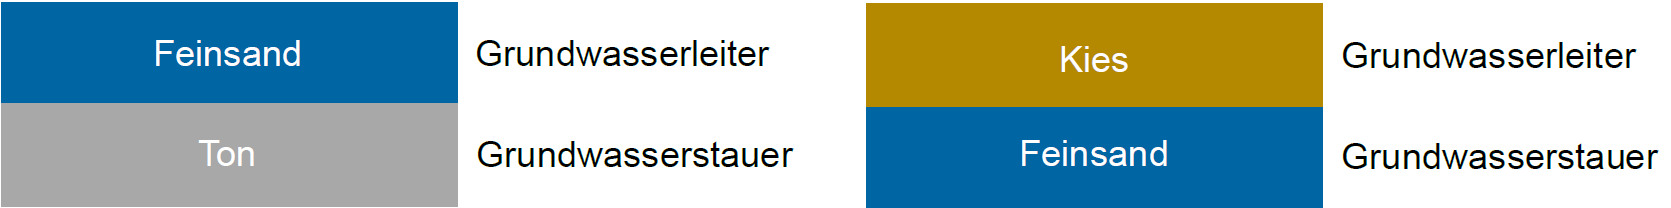
\includegraphics[width=\linewidth]{images/GW1Stauer.PNG} \\
%\end{minipage}
%\begin{minipage}{0.5\linewidth}
	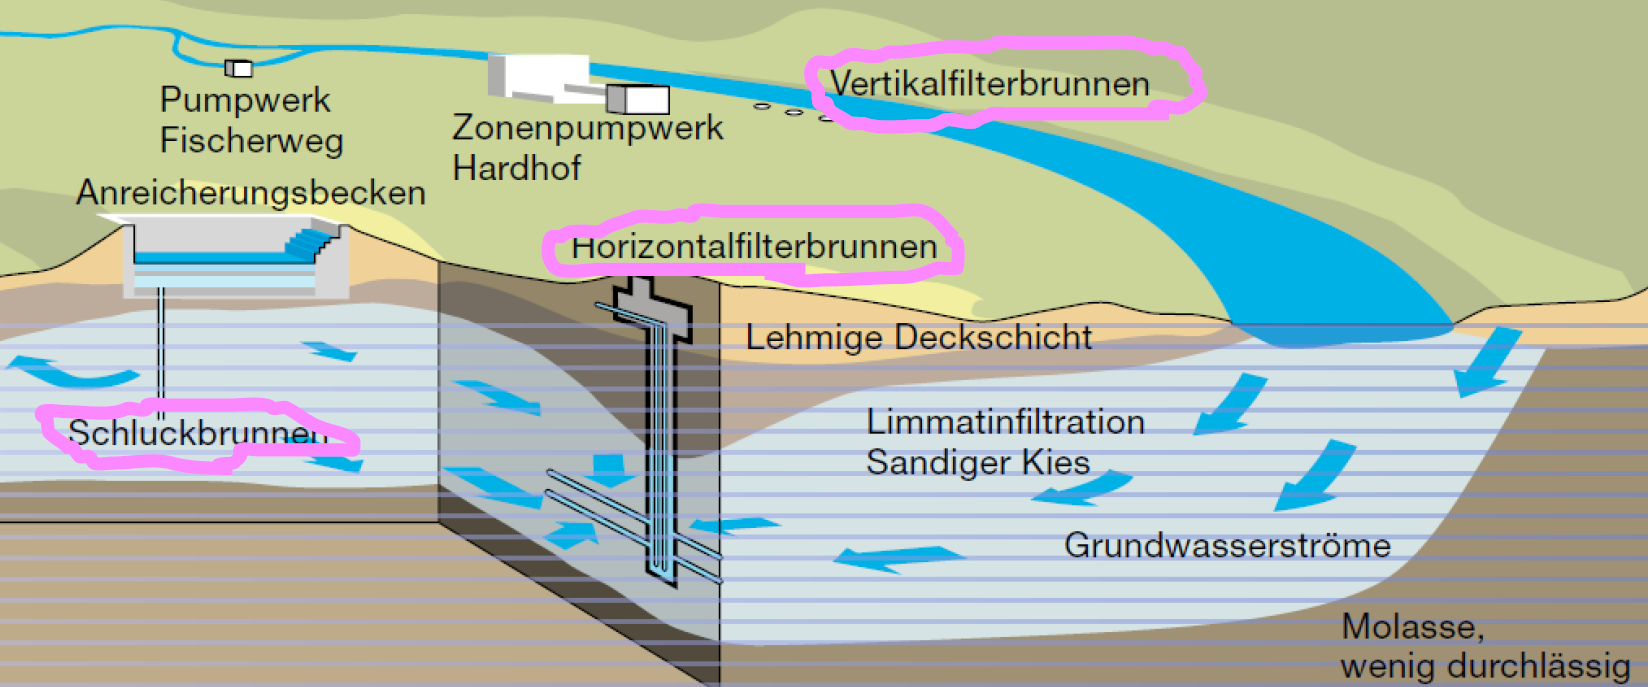
\includegraphics[width=0.9\linewidth]{images/GW2Fassung.PNG} \\
	
	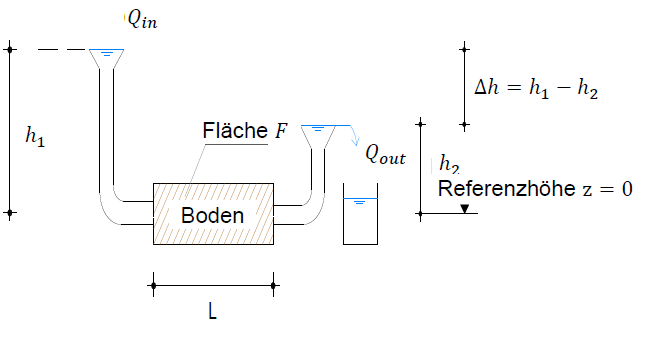
\includegraphics[width=\linewidth]{images/GW3Darcy.PNG} \\
\end{minipage}	
\begin{minipage}{0.7\linewidth}
	\subsection{Gesetz von Darcy}
	\begin{tabular}{p{0.25\linewidth}|l|p{0.4\linewidth}}
		Bemerkung	&	Formel			&	Def \\ \hline
		Bernoulli	&	$ h = z + \frac{u}{\gamma_w} $	&	h: Druckhöhe [m] \\
		Druckhöhe	&					& u: Porenwasserdruck [kPa] \\
					&					& z: Referenzhöhe [m.ü.M] \\ \hline
		Kontinuitätsgleichung	&	$ Q = v \cdot F $ 	& Q: Durchflussmenge [$ \frac{m^3}{s} $] \\
		Grundwasserleiter &					& v: Fliessgeschwindigkeit [ $ \frac{m}{s} $ ] \\ \hline
		Darcy		&  $ v = k \cdot\frac{\Delta h}{L} = k \cdot i $ &	i: hydraulischs Gefälle [-] \\
		Grundwasserleiter &				& k: Durchlässigkeitsbeiwert [ $ \frac{m}{s} $ ] \\
					&					& L: Durchströmte Länger [m] \\
					&					& $ \Delta $ h: Differenz der Druckhöhe [m] \\ \hline
		Wahre Geschwindigkeit eines Wasserteilchens &	$ v_{wahr} = \frac{v}{n} > v $	&	n: Porosität [-] \\
					&					& v: durchschnittliche Geschwindigkeit über ges. Bodenquerschnitt F \\
	\end{tabular}
%\end{minipage}
%\begin{minipage}{\linewidth}
	%	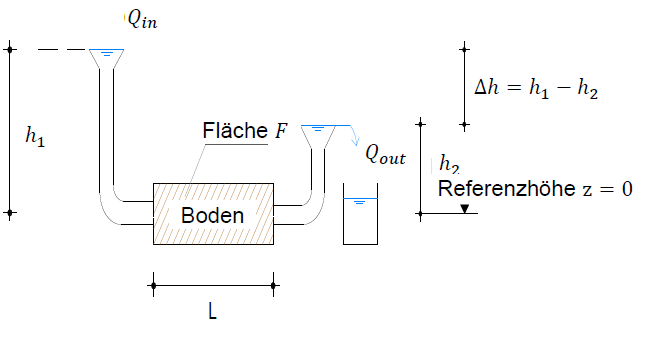
\includegraphics[width=\linewidth]{images/GW3Darcy.PNG} \\
\end{minipage}
\begin{minipage}{0.4\linewidth}
	\subsection{Durchlässigkeit k von Böden}
		
	Entwässerbarkeit:
	\begin{enumerate}
		\item gut wenn: k > 10$^{-3} \frac{cm}{s} $
		\item schlecht 10$^{-4}\frac{cm}{s} \geq k \geq 10^{-6} \frac{cm}{s} $
		\item undurchlässig k < 10$^{-6} \frac{cm}{s} $
	\end{enumerate}
\end{minipage}
\begin{minipage}{0.5\linewidth}
	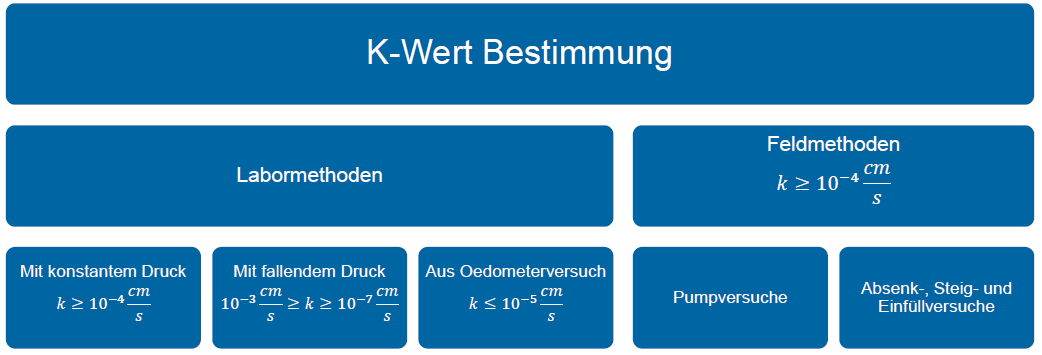
\includegraphics[width=\linewidth]{images/GW4Durchlaessigkeit.PNG} \\
\end{minipage}




\begin{landscape}


\begin{minipage}{0.5\linewidth}
	\subsubsection{Labor}
	
	\begin{tabular}{p{0.25\linewidth}|l|p{0.5\linewidth}}
		Bemerkung	& Formel			&	Def	 \\ \hline
		
		konstante Druckhöhe 	&	$ k = \frac{q \cdot L}{F \cdot \Delta h \cdot t} $	& q: Messvolumen Wasser [$m^3$] \\
		$ \rightarrow $ Sande/Kiese &	& t: Messperiode [s] \\ 
					&					& 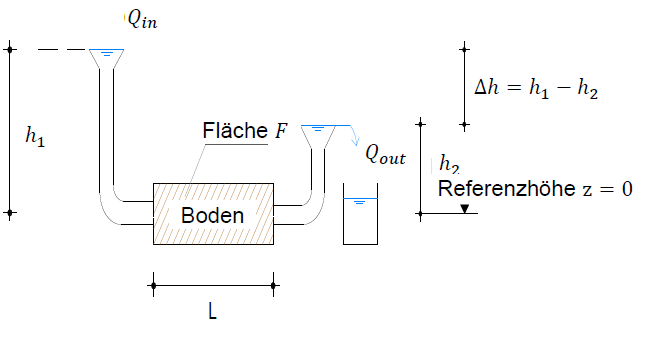
\includegraphics[width=\linewidth]{images/GW3Darcy.PNG} \\ \hline
		
		fallende Druckhöhe $ \rightarrow $ Silte	& $ k = \frac{a \cdot L}{F \cdot (t_2 - t_1) ln \frac{h_1}{h_2}} $	& \\
					&		& \vspace*{-1.25cm} 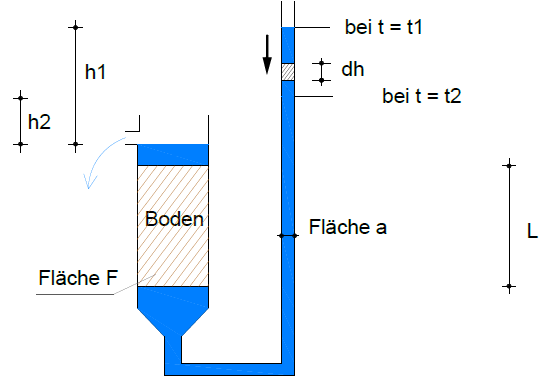
\includegraphics[width=0.8\linewidth]{images/GW5kfall.PNG} \\ \hline
		
		Zeit-Setzungskurve	& $ k = \frac{a_v \cdot \gamma_w \cdot 0.197 \cdot H^2}{(1 + e_m) t_{50}} $ & $a_v$: Verdichtungsbeiwert $ \frac{e_1 - e_2}{\sigma_1 - \sigma_2}$ \\
		$ \rightarrow $ Tone &			& $e_m$ : mittlere Porenziffer \\
					&					& 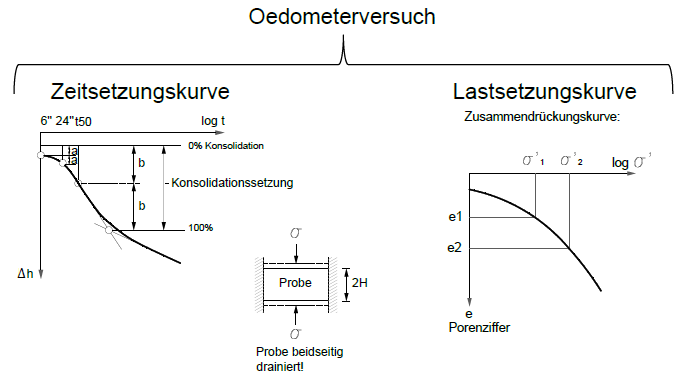
\includegraphics[width=\linewidth]{images/GW6Oedometer.PNG} \\
		
	\end{tabular}
\end{minipage}
\begin{minipage}{\linewidth}
	
	\subsubsection{Feld}
	
	
	\begin{tabular}{l|l|p{0.2\linewidth}}
		Bemerkung	& Formel			&	Def	 \\ \hline
		
		Pumpversuch nach Dupuit & $ k = \frac{Q}{\pi \cdot c} $ & $ c= \frac{H^2 - h_1^2}{ln \frac{R}{r_i} }$  \\
					&					& $ c = \frac{tan( \alpha ) }{2.3} $ \\
					&					& 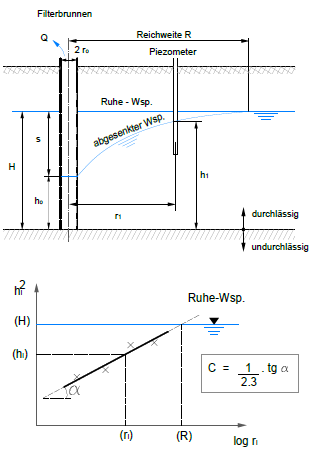
\includegraphics[width=\linewidth]{images/GW7Pump.PNG}  \\ \hline
		
		Pumpversuch nach Sichardt & $ R \widehat{\approx} 3000 \cdot s \sqrt{k} $ & R [m], s [m], k [ $ \frac{m}{s} $ ]  \\ \hline
		
		Absenk-/Steigversuch & $ k = c \frac{1}{h_m} \frac{\Delta h}{\Delta
		 t} $	& \smallskip 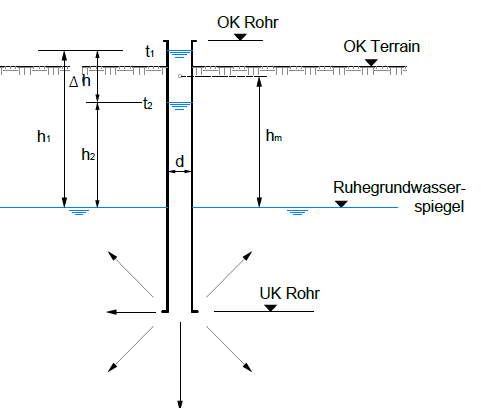
\includegraphics[width=\linewidth]{images/GW8Absenk.PNG}  \\ \hline
		
		Einfüllversuch & $ k = c \frac{1}{h} \frac{4Q}{\pi \cdot d^2} $  &\\
		
	\end{tabular}
\end{minipage}
%\begin{minipage}{\linewidth}
%	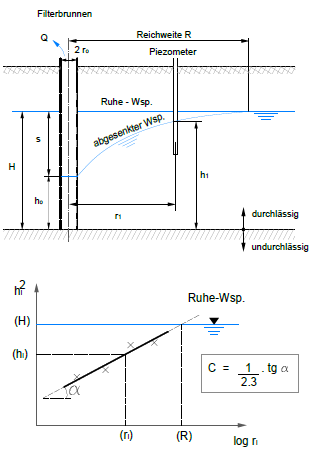
\includegraphics[width=0.35\linewidth]{images/GW7Pump.PNG} \\
%	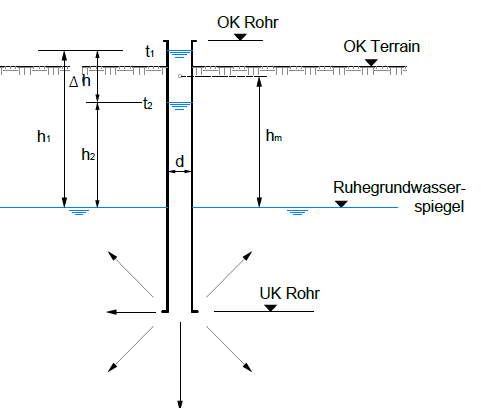
\includegraphics[width=0.35\linewidth]{images/GW8Absenk.PNG} \\
%\end{minipage}

%\end{landscape}



%\begin{minipage}{0.6\linewidth}
%\subsection{Absenkbrunnen}
%	
%	\begin{itemize}
%		\item Offene Wasserhaltung: kleine Bauvorhaben, geringe Absenkung
%		\item Kleine Filterbrunnen: kleinere Bauvorhaben, durchlässige Böden
%		\item Grosse Filterbrunnen: grosse Bauvorhaben, durchlässige Böden
%		\item Wellpoint:kleine bis grosse Bauvorhaben, undurchlässige Böden (min 1.5 m Abstand zwischen Lanzen)
%		
%	\end{itemize}
%
%%\end{minipage}
%%
%%\begin{minipage}{0.5\linewidth}
%		\begin{tabular}{p{0.3\linewidth}|l|p{0.25\linewidth}}
%					
%			\multicolumn{3}{c|}{ \textbf{ungespannter Aquifer} } \\ \hline
%			
%			Vollkommener Vertikalbrunnen (Dupuit-Thiem) & $ Q = \pi \cdot k \frac{H^2 - h_0^2}{ln \frac{R}{r_0} } $	& \smallskip 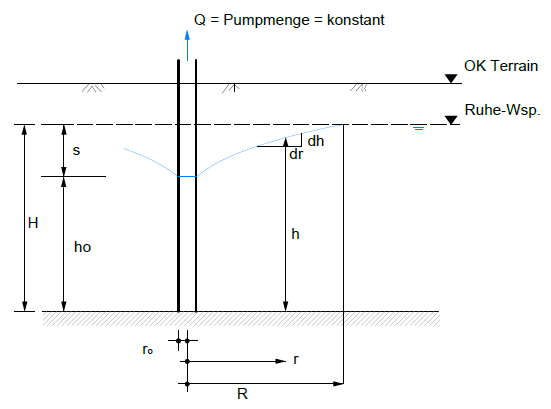
\includegraphics[width=\linewidth]{images/GW9ungespAquifer.PNG}  \\
%			Filterergiebigkeit & $ v_{Grenz} \hat{\approx} \frac{\sqrt{k}}{15}$	& [ $ \frac{m}{s} $ ] \\ \hline
%			
%			\multicolumn{3}{c|}{ \textbf{gespannter Aquifer} } \\ \hline
%			
%			Vollkommener Vertikalbrunnen (Dupuit-Thiem) & $ Q = 2 \cdot \pi \cdot m \cdot k \frac{H - h_0}{ln \frac{R}{r_0} } $	& \smallskip 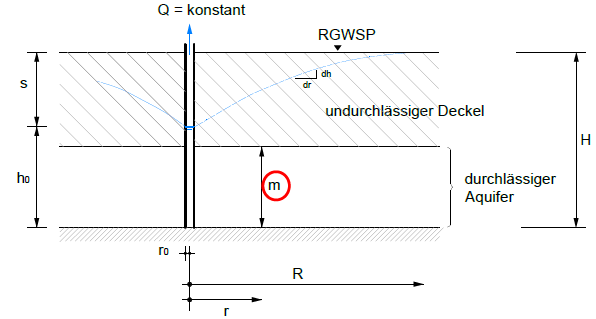
\includegraphics[width=\linewidth]{images/GW10gespAquifer.PNG}  \\ \hline
%			
%			Unvollkommener Vertikalbrunnen (der Brunnen reicht nicht bis zur undurchlässigen Stauschicht)	& $ Q_{unvollk} \approx (1.1 \div 1.3) \cdot Q_{vollk} (H = H_1) $	& \smallskip 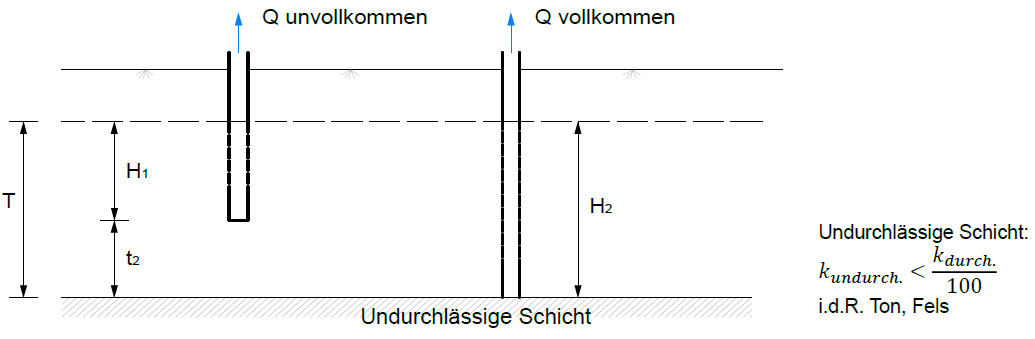
\includegraphics[width=\linewidth]{images/GW11gespAquiferunvollk.PNG}  \\
%						
%		\end{tabular}
%	\end{minipage}
%	\begin{minipage}{0.4\linewidth}
%		
%		\subsubsection{Weitere Grundwasseranwendungen}
%		
%		\begin{tabular}{p{0.3\linewidth}|p{0.35\linewidth}|p{0.3\linewidth}}
%			Bemerkung 		& Formel			&	Einheit \\ \hline
%			
%			Zufluss zu Bach (ungespannt) & $ Q = k \frac{H^2 - L^2}{r \cdot R} $	& \smallskip 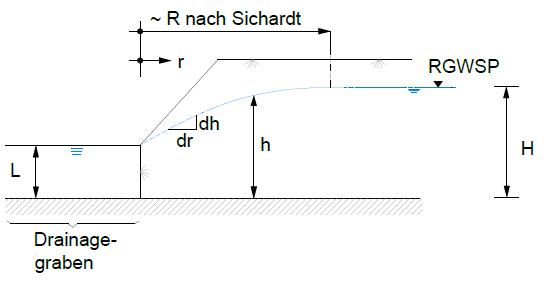
\includegraphics[width=\linewidth]{images/GW12Bachungespannt.PNG}  \\ \hline
%			
%			Zufluss zu Bach (gespannt)	& $ Q = m \cdot k \frac{H - L}{R} $ & \smallskip 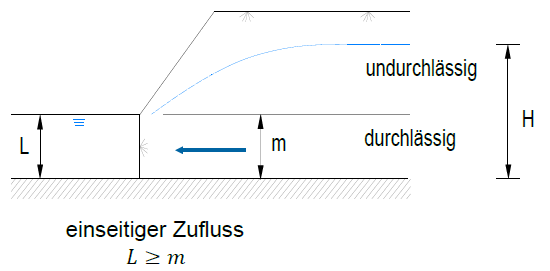
\includegraphics[width=\linewidth]{images/GW13Bachgespannt.PNG}  \\ \hline
%			
%			GW-Absenkung für Baugrube mit mehreren Brunnen 	& 1. Fiktiver Radius R$_A = \sqrt{\frac{a \cdot b}{\pi} } $ [m]	& R$_A$ : fiktiver Radius (Baugrubenabmessung a x b) $ R_A = \sqrt{ \frac{a \cdot b }{\pi} } $ \\
%															& 2. Abschätzung Pumpwassermenge Q$_{tot} =\pi \cdot k \frac{H^2 - h^2}{ln(R) - ln(R_A) } $ [$ \frac{m^3}{s} $]												& \smallskip \multirow{7}{*}{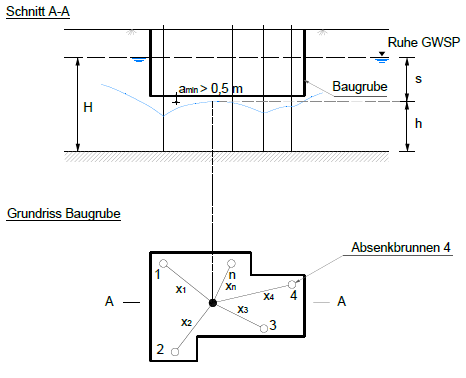
\includegraphics[width=\linewidth]{images/GW14mehrereBrunnen.PNG} }  \\
%															& 3. v$_{Grenz} = \frac{ \sqrt{k} }{15} $ [$ \frac{m}{s} $]		& \\
%															& 4. erf. benetzte Brunnenmantelfläche $ M_{erf} = \frac{Q_{tot} }{v_{Grenz} } [m^2]$ & \\
%															& 5. Filterhöhe $ h = \frac{M_{erf} }{U_{Brunnen} } $ [m] $ \rightarrow $ Faktor 2 Sicherheit bei Anzahl Brunnen												& \\
%															& 6. GW-Spiegelhöhe z an beliebiger Stelle $ z = \sqrt{ H^2 - \frac{Q_{tot} }{\pi \cdot k} [ln(R) - \frac{1}{n} ln(x_i) ] } $								& \\
%															& 7. Pumpwassermenge an beliebiger Stelle Q$_{f} = \pi \cdot k \frac{H^2 - z^2 }{ln(R) - \frac{1}{n} ln(x_1 \cdot x_2 \cdot ... x_n) } $					& \\
%															& 8. Pumpwassermenge pro Brunnen Q$_{erf} = \frac{Q_f}{n} $		& \\
%%			\begin{enumerate}
%%				\item Fiktiver Radius R$_A = \sqrt{\frac{a \cdot b}{\pi} } $ [m]
%%				\item Abschätzung Pumpwassermenge Q$_{tot} =\pi \cdot k \frac{H^2 - h^2}{ln(R) - ln(R_A) } $ [$ \frac{m^3}{s} $]
%%				\item v$_{Grenz} = \frac{ \sqrt{k} }{15} $ [$ \frac{m}{s} $]
%%				\item erf. benetzte Brunnenmantelfläche $ M_{erf} = \frac{Q_{tot} }{v_{Grenz} } [m^2]$
%%				\item Filterhöhe $ h = \frac{M_{erf} }{U_{Brunnen} } $ [m] $ \rightarrow $ Faktor 2 Sicherheit bei Anzahl Brunnen
%%				\item GW-Spiegelhöhe z an beliebiger Stelle $ z = \sqrt{ H^2 - \frac{Q_{tot} }{\pi \cdot k} [ln(R) - \frac{1}{n} ln(x_i) ] } $
%%				\item Pumpwassermenge an beliebiger Stelle Q$_{f} = \pi \cdot k \frac{H^2 - z^2 }{ln(R) - \frac{1}{n} ln(x_1 \cdot x_2 \cdot ... x_n) } $
%%				\item Pumpwassermenge pro Brunnen Q$_{erf} = \frac{Q_f}{n} $
%%			\end{enumerate}
%%		& R$_A$ : fiktiver Radius (Baugrubenabmessung a x b) $ R_A = \sqrt{ \frac{a \cdot b }{\pi} } $ \\
%%							&					& \smallskip 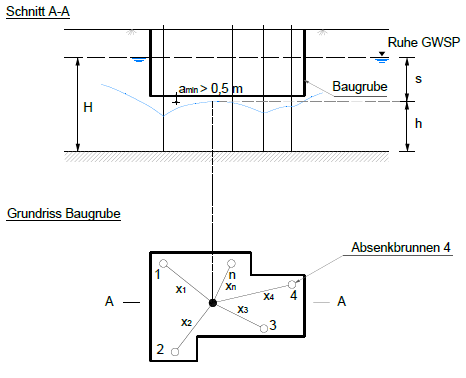
\includegraphics[width=\linewidth]{images/GW14mehrereBrunnen.PNG}  \\ \hline
%			
%		\end{tabular}
%	\end{minipage}

\end{landscape}

\begin{minipage}{\linewidth}
	\vspace{-0.5cm}
	\subsection{Absenkbrunnen}
	
	\begin{itemize}
		\item Offene Wasserhaltung: kleine Bauvorhaben, geringe Absenkung
		\item Kleine Filterbrunnen: kleinere Bauvorhaben, durchlässige Böden
		\item Grosse Filterbrunnen: grosse Bauvorhaben, durchlässige Böden
		\item Wellpoint:kleine bis grosse Bauvorhaben, undurchlässige Böden (min 1.5 m Abstand zwischen Lanzen)
		
	\end{itemize}
	
	%\end{minipage}
	%
	%\begin{minipage}{0.5\linewidth}
	\begin{tabular}{p{0.3\linewidth}|l|p{0.25\linewidth}}
		
		\multicolumn{3}{c|}{ \textbf{ungespannter Aquifer} } \\ \hline
		
		Vollkommener Vertikalbrunnen (Dupuit-Thiem) & $ Q = \pi \cdot k \frac{H^2 - h_0^2}{ln \frac{R}{r_0} } $	& \multirow{2}{*}{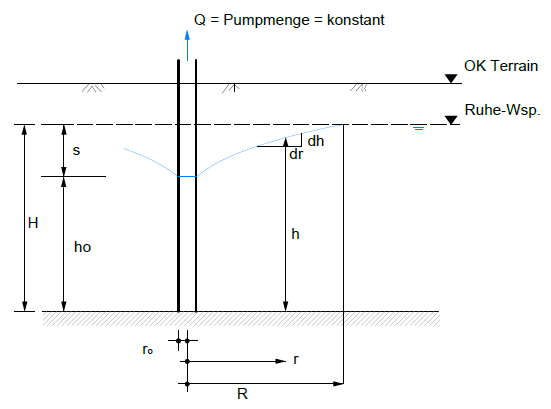
\includegraphics[width=0.8\linewidth]{images/GW9ungespAquifer.PNG}}  \\
		Filterergiebigkeit & $ v_{Grenz} \hat{\approx} \frac{\sqrt{k}}{15}$	&\\ \hline
		
		\multicolumn{3}{c|}{ \textbf{gespannter Aquifer} } \\ \hline
		
		Vollkommener Vertikalbrunnen (Dupuit-Thiem) & $ Q = 2 \cdot \pi \cdot m \cdot k \frac{H - h_0}{ln \frac{R}{r_0} } $	& \smallskip 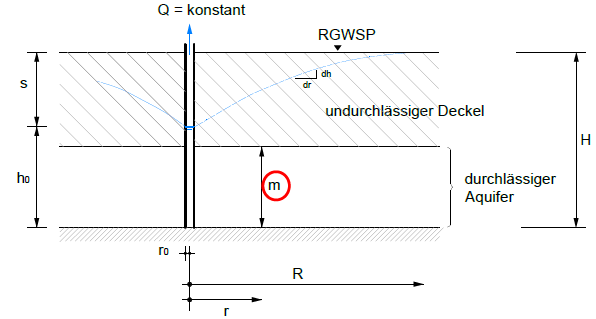
\includegraphics[width=0.8\linewidth]{images/GW10gespAquifer.PNG}  \\ \hline
		
		Unvollkommener Vertikalbrunnen (der Brunnen reicht nicht bis zur undurchlässigen Stauschicht)	& $ Q_{unvollk} \approx (1.1 \div 1.3) \cdot Q_{vollk} (H = H_1) $	& \smallskip 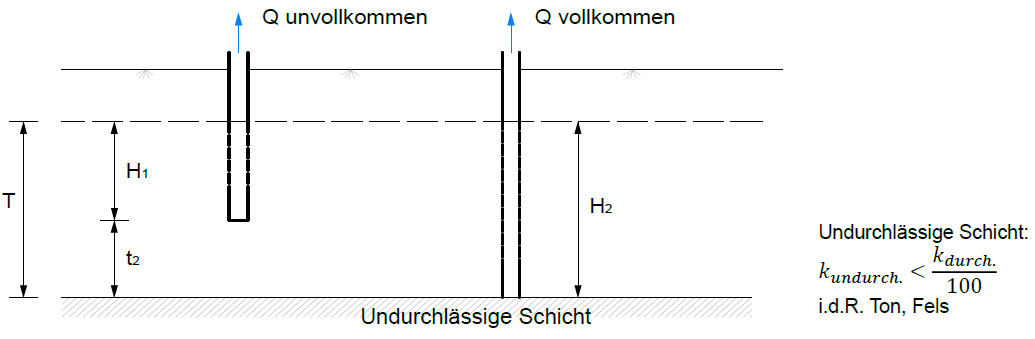
\includegraphics[width=\linewidth]{images/GW11gespAquiferunvollk.PNG}  \\
		
	\end{tabular}
\end{minipage}
\begin{minipage}{\linewidth}
	
	\subsubsection{Weitere Grundwasseranwendungen}
	
	\begin{tabular}{p{0.2\linewidth}|p{0.5\linewidth}|p{0.25\linewidth}}
		Bemerkung 		& Formel			&	Einheit \\ \hline
		
		Zufluss zu Bach (ungespannt) & $ Q = k \frac{H^2 - L^2}{r \cdot R} $	& \smallskip 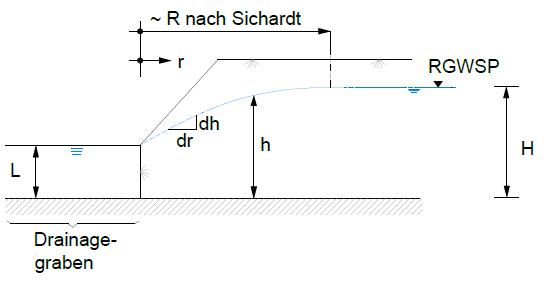
\includegraphics[width=\linewidth]{images/GW12Bachungespannt.PNG}  \\ \hline
		
		Zufluss zu Bach (gespannt)	& $ Q = m \cdot k \frac{H - L}{R} $ & \smallskip 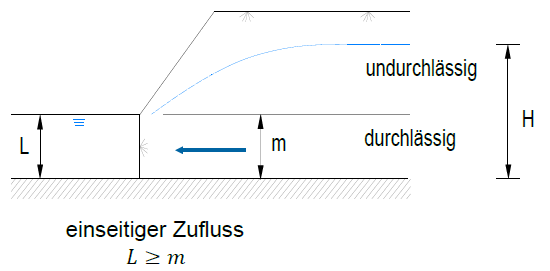
\includegraphics[width=\linewidth]{images/GW13Bachgespannt.PNG}  \\ \hline
		
		GW-Absenkung für Baugrube mit mehreren Brunnen 	& 1. Fiktiver Radius R$_A = \sqrt{\frac{a \cdot b}{\pi} } $ [m]	& R$_A$ : fiktiver Radius (Baugrubenabmessung a x b) $ R_A = \sqrt{ \frac{a \cdot b }{\pi} } $ \\
		& 2. Abschätzung Pumpwassermenge Q$_{tot} =\pi \cdot k \frac{H^2 - h^2}{ln(R) - ln(R_A) } $ [$ \frac{m^3}{s} $]												& R = 3000 $\cdot$ s $\cdot$ $\sqrt{k}$ \smallskip \multirow{7}{*}{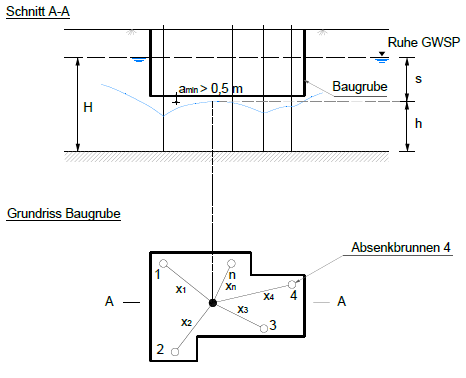
\includegraphics[width=\linewidth]{images/GW14mehrereBrunnen.PNG} }  \\
		& 3. v$_{Grenz} = \frac{ \sqrt{k} }{15} $ [$ \frac{m}{s} $]		& \\
		& 4. erf. benetzte Brunnenmantelfläche $ M_{erf} = \frac{Q_{tot} }{v_{Grenz} } [m^2]$ & \\
		& 5. Filterhöhe $ h = \frac{M_{erf} }{U_{Brunnen} } $ [m] $ \rightarrow $ Faktor 2 Sicherheit bei Anzahl Brunnen												& \\
		& 5.1 Anzahl Brunnen $ n = \frac{Q_{tot}}{v_{Grenz} \cdot U_B \cdot h} $	& \\
		& 6. GW-Spiegelhöhe z an beliebiger Stelle über undurchlässige Schicht $ z = \sqrt{ H^2 - \frac{Q_{tot} }{\pi \cdot k} [ln(R) - \frac{1}{n} ln(x_i) ] } $								& \\
		& 7. Pumpwassermenge an beliebiger Stelle Q$_{f} = \pi \cdot k \frac{H^2 - z^2 }{ln(R) - \frac{1}{n} ln(x_1 \cdot x_2 \cdot ... x_n) } $					& \\
		& 8. Pumpwassermenge pro Brunnen Q$_{erf} = \frac{Q_f}{n} $		& Sandfreiheit: $ Q = A_{Filter} v_{Grenz} $ \\
		
	\end{tabular}
\end{minipage}

%\clearpage

	\begin{minipage}{\linewidth}
		
		\subsubsection{Sickernetze}
		
		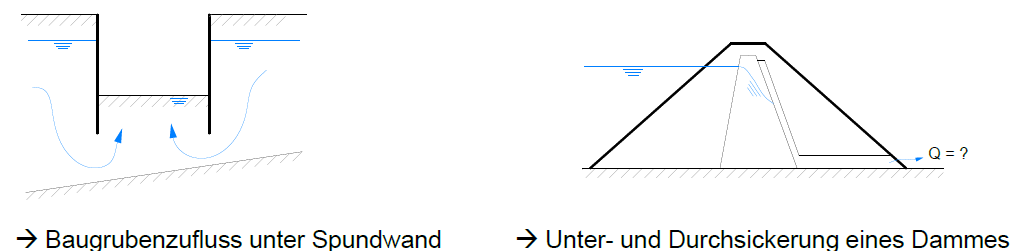
\includegraphics[width=0.6\linewidth]{images/GW15Sickerwassermenge.PNG}
		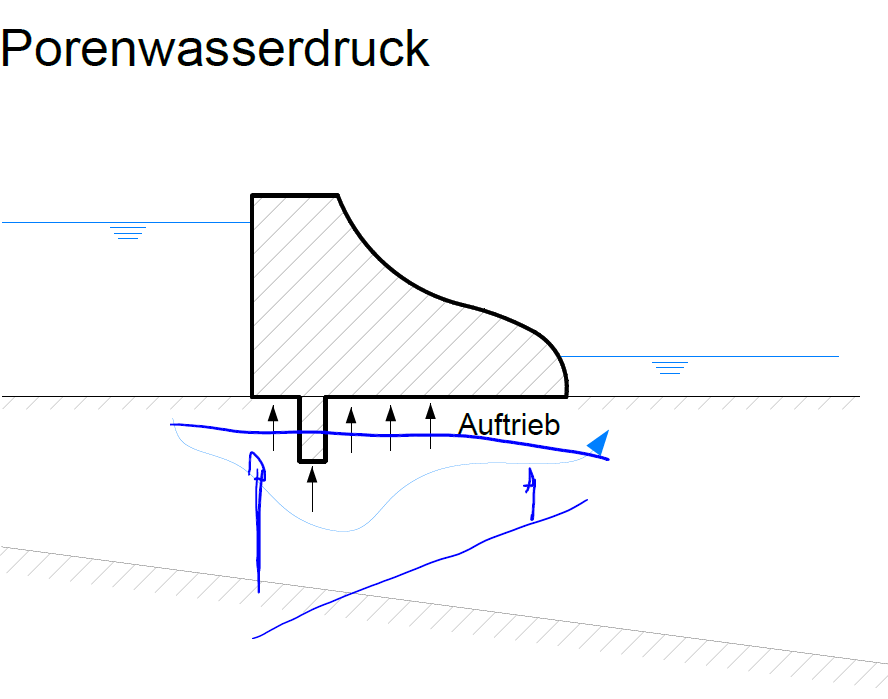
\includegraphics[width=0.2\linewidth]{images/GW16Porenwasserdruck.PNG}		\\
	\end{minipage}
\begin{minipage}{0.5\linewidth}
		
		\textbf{Konstruktion von Sickernetzen}
		\begin{enumerate}
			\item QS aufzeichnen (Massstab, mögl. quadratisch)
			\item Begrenzung einzeichnen (undurchlässige Schichten, Bäche, Seen)
			\item Sickernetz konstruieren (Potentiallinien, Stromlinien)
					$ \rightarrow $ N$_f$ = Anzahl Stromröhren (in jeder Stromröhre fliesst gleichviel GW); N$_d$ = Anzahl Potentialstufen (auf einer Potentiallinie ist gleicher Wasserdruck/gl. Piezometerhöhe)
			\item Formeln:			
		\end{enumerate}
		\begin{itemize}
			\item Durchfluss pro Rohr: $ \Delta Q = k \cdot \frac{\Delta H}{\Delta L} \cdot \Delta b $
			\item $ v = k \cdot i $
			\item $ i = \frac{\Delta H}{\Delta L} $
			\item $ Q = N_f \cdot \Delta Q $
			\item $ H = N_d \cdot \Delta H $
			\item $ Q = k \cdot H \cdot \frac{N_f}{N_d} $ [ $ \frac{m^3}{s \cdot m^l} $ ]
			\item Wasserdruck/Piezometer: $ h = H - \frac{H}{N_d} \cdot n $ [m] $ \rightarrow \cdot 10 = u [\frac{kN}{m^2}] $; wobei n = Anzahl Felder
			\item Auftrieb: $ A = u \cdot L \cdot B $ [kN]
			\item Nachweis: $ 1.1 \cdot A \leq G $
		\end{itemize}
	
\end{minipage}
\begin{minipage}{0.4\linewidth}
	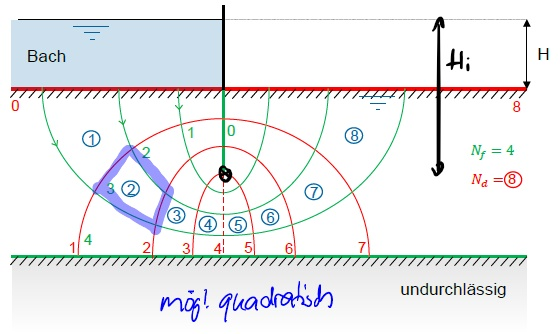
\includegraphics[width=\linewidth]{images/GW17Sickernetz.jpg}
\end{minipage}





\begin{minipage}{0.7\linewidth}
	
	\subsubsection{Hydraulischer Grundbruch}
	
	\begin{tabular}{p{0.23\linewidth}|l|l}
				
		\multicolumn{3}{c}{\textbf{Strömungsdruck} } \\ \hline
		
		Strömungsgradient &	$ i_{vorh} = \frac{\Delta H}{t} $	& $\Delta$ H: Absenkung GW [m] \\
					&	$ i_{vorh,isotrop} = \frac{\Delta H}{\Delta H + 2 \cdot t} $				& t: Einbindetiefe [m] \\
					&	$ i_{krit} = \frac{\gamma'}{\gamma_w} $	& \\
		Sicherheit  &	$ F = \frac{i_{krit} }{i_{vorh} } $	& auflösen nach t [m] \\ 
					&	& F$_H$ $\geq$ 4.5 $\rightarrow$ Isotroper Boden \\ 
					&	& F$_H$ $\geq$ 1.5 $\rightarrow$ Anisotroper Boden \\ \hline
		
		Einbindetiefe anisotropisches Zuströmen neues Konzept nach SIA 267 &	$ \gamma' \cdot \gamma_{G,inf} \geq \gamma_w \cdot i_{vorh} \cdot \gamma_{G,sup} $	& $\gamma_{G}$: Sia 260, Tab. 1	\\
		
		Porenwasserdruck & $ u = u_0 - \Delta u = u_0 - i \cdot \gamma_w \cdot z $ & \\
		
		Effektive Spannung & $ \sigma_v' = \sigma_v - u = \sigma_{v,0}' + \Delta u $	& \\
		
		Gewicht Bodenelement unter Auftrieb & $ G = \gamma' \cdot A $	& \\
		
		Strömungskraft	& $ S = \gamma_w \cdot i \cdot A $	& \\
		
		Resultierende Auf-/Abwärtsströmung & $ R = (\gamma' \pm \gamma_w \cdot i) \cdot V $	& \\ \hline
		
		Sicherheit	& $ F = \frac{G}{S} $	& \\
		
		
		\multicolumn{3}{c}{\textbf{Wasserdrücke im Boden} } \\ \hline
		
		hydrostatischer Druck	& $ w = \gamma_w \cdot t $	&	\\
		
		mit Aufwärtsströmung	& $ w = \gamma_w (1 + i) t $	& \\
		
		mit Abwärtsströmung		& $ w = \gamma_w (1 - i) t $	& \\
		
		seitliche Kraft aus Wasserdruck & $ W = 0.5 \cdot t \cdot w = 0.5 \cdot t^2 \cdot \gamma_w $	& [ $ \frac{kN}{m^l} $ ] \\
		
		Auftriebkraft	& $ A = w \cdot b = t \cdot b \cdot \gamma_w $ & [ $ \frac{kN}{m^l} $ ] \\
		
		Bemesseung		& $ G \geq F_s \cdot A $	& F$_s = \frac{\gamma_{G,sup}}{\gamma_{G,inf}} \geq 1.1 \div 1.2 $ \\
		
		
	\end{tabular}
\end{minipage}
\begin{minipage}{0.3\linewidth}
	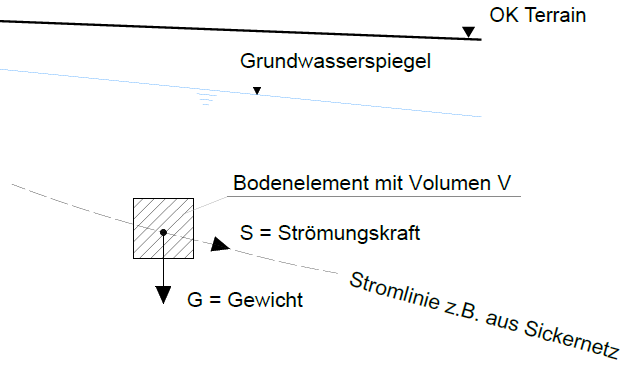
\includegraphics[width=\linewidth]{images/GW18Kraftwirkung.PNG}
	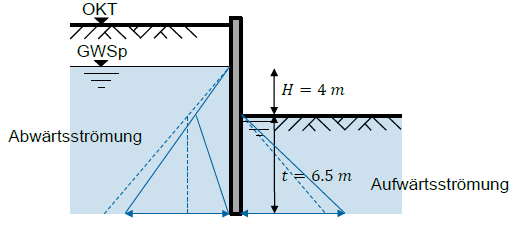
\includegraphics[width=\linewidth]{images/GW19Stroemungsdruck.PNG}
%	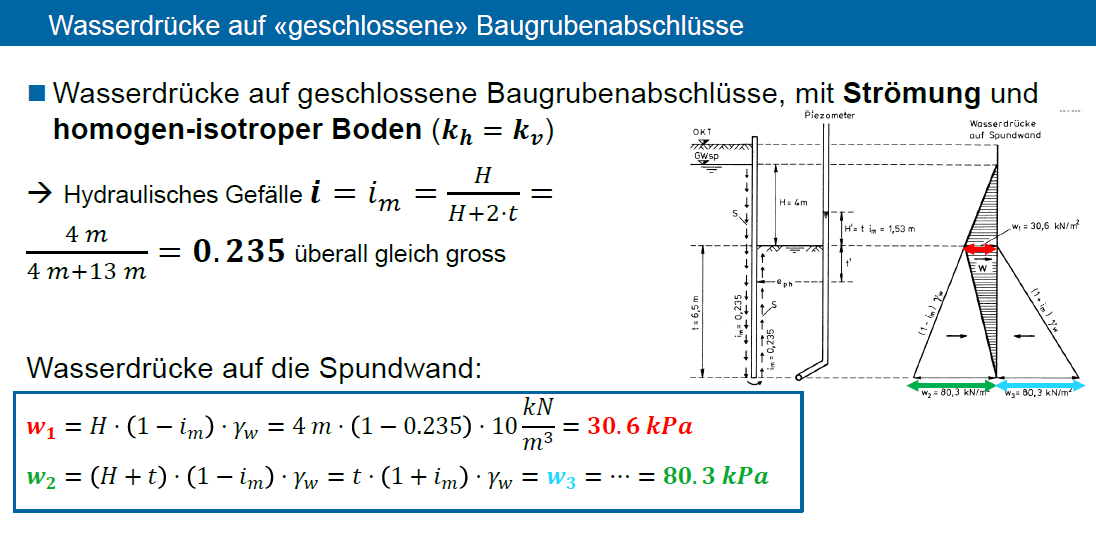
\includegraphics[width=\linewidth]{images/GW20Wasserdrucke.PNG}
	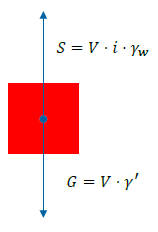
\includegraphics[width=0.5\linewidth]{images/GW21Kraftwirkung.PNG}
\end{minipage}
	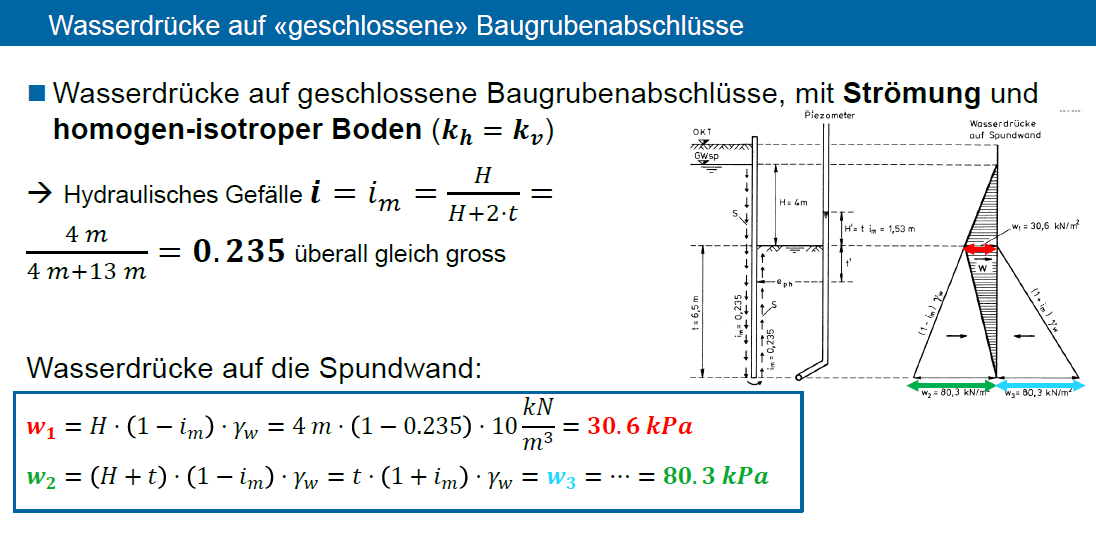
\includegraphics[width=0.8\linewidth]{images/GW20Wasserdrucke.PNG}